\newpage
\section{Implementierung}
Wie in Abschnitt XX bereits erwähnt ist die Applikation dem Design-Pattern Model-View-Controller nachempfunden. Im Folgenden wird nun die konkrete Implementierung beschrieben und die Architektur mittels Codebeispielen konkretisiert.
\\
Der allgemeine Ablauf der Anwendung sieht lediglich einen Aufruf der HTML-Seite index.html vor. In diese wird mittels Javascript der jeweilige Inhalt (eine View) geladen und mit Daten und Funktionen (Controller) und versorgt.
\\
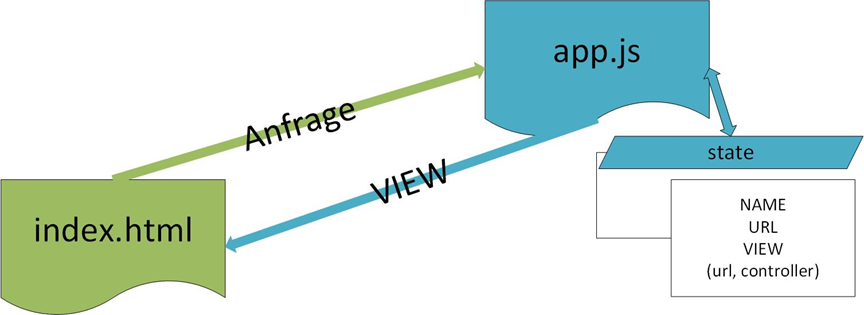
\includegraphics[width=1\textwidth]{ref/images/index.png} \\ 
App.js ist eine Javascript-Datei, die die Zuordnung der Views zu ihrem jeweiligen Controller durchführt. An dieser Stelle ist pro View ein Status (state) hinterlegt, der die Informationen hält (Name des Status, URL (innerhalb der App), View-Bezeichnung (URL der View, Controllername)). Die Informationen über die aktuell gewählte View gibt app.js an index.html zurück, welche sie nach außen dem Nutzer darstellt.
\\
App.js wird bei jedem Start der Applikation zuerst geladen. Dabei findet auch immer eine Prüfung der aktuellen Internetverbindung statt.
\\
Internet wird für die Darstellung des Kartenmaterials benötigt. Die Konsequenz einer fehlenden Internetverbindung ist demnach ein Abbruch der Applikation.
\\
Standardmäßig wird bei korrektem Startverhalten die play-View geladen. Das ist eine ebenfalls in App.js definierte Defaulteinstellung.
\\
Alle folgenden Statusbeschreibungen trennen View, Controller und Modell schematisch voneinander, wobei der Begriff Modell durch den Cordova-spezifischen Begriff Service ersetzt wird.
\\
Die App besitzt einen getabbten Aufbau, das heißt es existiert eine Kopfzeile, die dem Nutzer 4 verschiedene Tabs anbietet: Spielen, Highscores, Account und Credits. Jeder der Tabs wird im Folgenden näher beschrieben werden.
\subsection{Spielen}
Der Spielen-Tab bietet dem Nutzer die Möglichkeit sich für ein Spiel anzumelden. Er gibt dafür einen Namen und einen Spielradius an. Unter dieser Kombination wird er später seinen Highscore dieses Spiels finden können. Die View, die dahinter steht ist die Play-View, welche prinzipiell als Startseite der Applikation angezeigt wird. Sie hat ein Textfeld, dass den Spielernamen übernehmen kann und eine Selectbox, die den Radius auf zwei bis fünf Kilometern beschränkt. Bei fehlender Eingabe wird auf drei Kilometer als Defaultwert gesetzt. Außerdem bietet die View einen Button, der das Spiel startet. 
\\
Schon während der Eingabe der benötigten Informaitonen (Name und Radius) wird ein Objekt 'player' generiert, des diese Daten enthält, und mit Druck auf den Button an die Funktion savePlayer übergeben wird. Die Funktion 'savePlayer(p)' wurde der View durch den Controller 'PlayCtrl' (zugewiesen über app.js) bereitgestellt.
\\
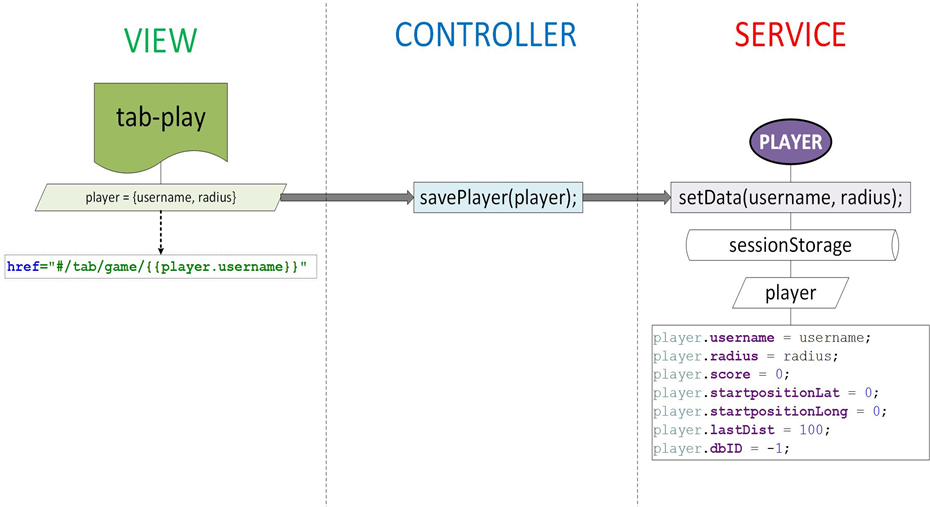
\includegraphics[width=1\textwidth]{ref/images/play.png} \\ 
\\
Der Controller leitet bei Aufruf dieser Funktion die Objektdaten Name und Radius an den dazugehörigen Service 'Player', der zuerst auf gültige Befüllung des Spielernamen prüft und bei Befüllung diesen speichert.